\chapter{Algumas verificações e validações}\label{Algumas_verificacoes_validacoes}

\section{Validação referente a parte elastoplástica através de um ensaio}

Uma vez que se tem um ensaio triaxial, como por exemplo, o da \autoref{ensaio_triaxial_ductil} uma validação do endurecimento e amolecimento da parte elastoplástica é possível. Os modelos estão apresentados na \autoref{malha_ensaio_triaxial} e compreendem a simulação numérica de um ensaio considerando um modelo 3D, estado plano de deformação e axissimétrico. Sendo $l_a = l_b = l_c = 1$ o próprio deslocamento em y do nó A será a deformação específica. Para representar o ensaio foi aplicado um deslocamento imposto $\delta = 0.1$ na face superior.

\begin{figure}[H]
	\begin{center}
		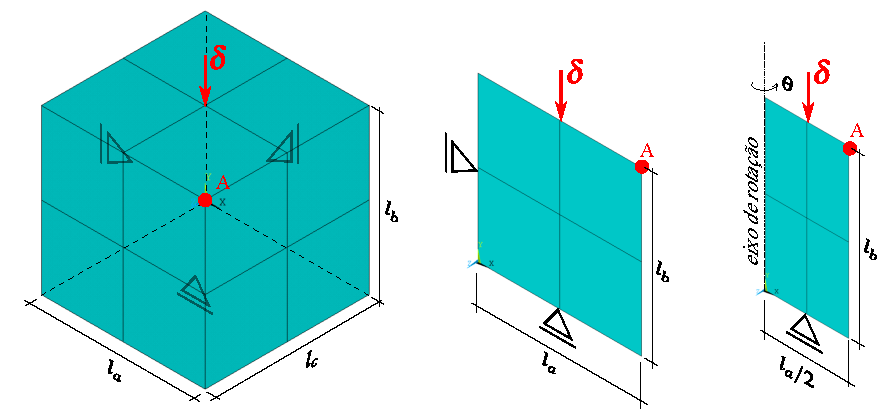
\includegraphics[scale = 1.0]{0701-Malha_ensaio_triaxial.pdf}
	\end{center}
	\caption{\label{malha_ensaio_triaxial}Domínio e discretização de um ensaio triaxial com modelo 3D, EPD e AXI}
\end{figure}

Os valores dos parâmetros do modelo constitutivo adotado na análise foram $E = 403$MPa, $\nu = 0.39$,  superficief = 2, superficieg = 2, $\phi = 0, \psi = 0, c_i = 0,7, c_p = 1,3, c_r = 0,9, \bar \varepsilon^p_{I} = 0,010, \bar \varepsilon^p_{II} = 0,050, \bar \varepsilon^p_{r} = 0,07$, Dalg = 0. Os parâmetros de coesão e de deformação plástica equivalente das zonas de endurecimento e amolecimento são coletadas do gráfico do ensaio, tal como apresentado na \autoref{ensaio_triaxial_parametros}. O valor de duas vezes a coesão está no fato de que não está sendo considerado o ângulo de atrito e de dilatância, fazendo com que a superfície de plasticidade se reduza a de von-Mises. Nesse aspecto, a variação do volume não considera a dilatância durante a deformação plástica. A parte viscosa do modelo constitutivo é eliminada utilizando uma coesão alta. O resultado da análise pode ser visto na \autoref{ensaio_triaxial_solucao}.
 
\begin{figure}[H]
 	\begin{center}
 		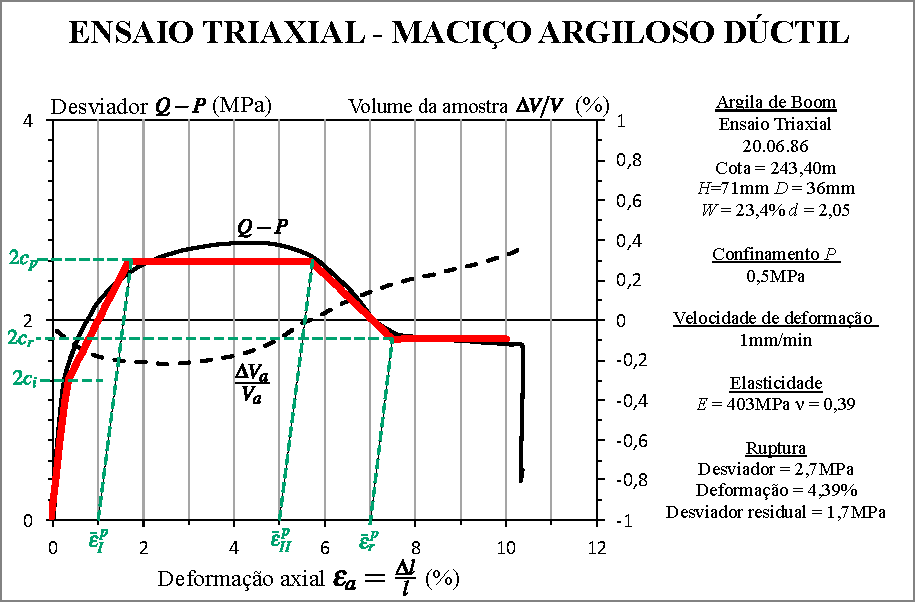
\includegraphics[scale = 1.0]{0702-ensaio triaxial argila ductil_coletando_parametros.pdf}
 	\end{center}
 	\caption{\label{ensaio_triaxial_parametros}Domínio e discretização de um ensaio triaxial com modelo 3D, EPD e AXI}
\end{figure}

\begin{figure}[H]
	\begin{center}
		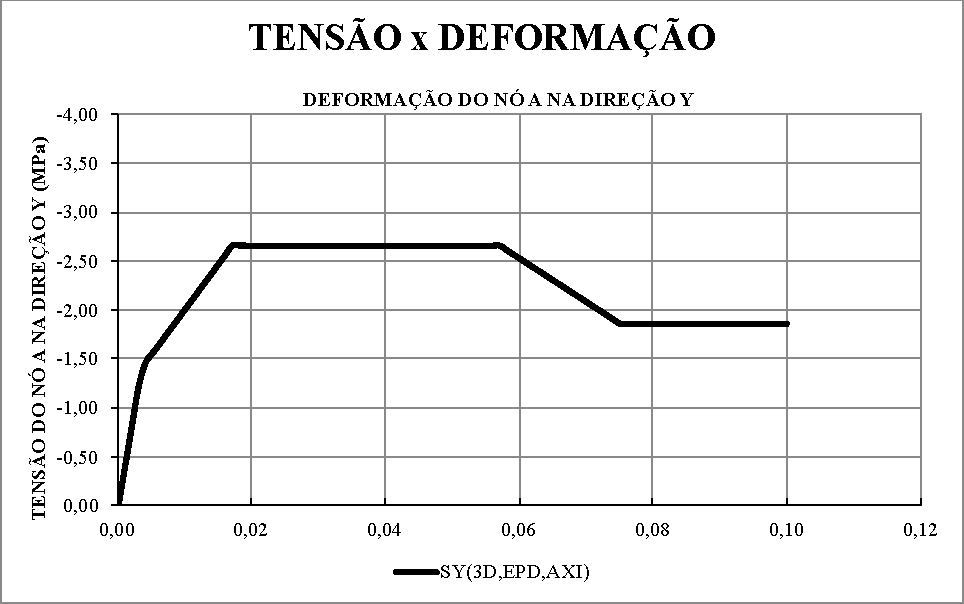
\includegraphics[scale = 1.0]{0703-ensaio triaxial argila ductil solucao.pdf}
	\end{center}
	\caption{\label{ensaio_triaxial_solucao}Resultado da análise para o ensaio triaxial}
\end{figure}

Como pode-se ver os valores deram exatamente iguais considerando 3D, EPD e AXI demonstrando que a implementação conseguiu essa generalidade. Caso o modelo seja de fato utilizado para estudos de túneis reais é sempre desejável ter ensaios triaxiais para fazer a validação ou eventuais calibrações nesse aspecto do modelo.

\section{Verificação da solução numérica com uma solução analítica considerando o endurecimento}
